\RequirePackage{currfile}
\documentclass[12pt]{beamer}
\usepackage[utf8]{inputenc}
\usepackage[spanish]{babel}
\usepackage{standalone}
\usepackage{color}
\usepackage{siunitx}
\usepackage{hyperref}
%\hypersetup{colorlinks,linkcolor=,urlcolor=blue}
%\hypersetup{colorlinks,urlcolor=blue}
\usepackage{xcolor,soul}
\usepackage{etoolbox}
\usepackage{amsmath}
\usepackage{amsthm}
\usepackage{physics}
\usepackage{multicol}
\usepackage{bookmark}
\usepackage{longtable}
\usepackage{listings}
\lstset{
basicstyle=\ttfamily,
columns=fullflexible,
breaklines=true
}
\usepackage{graphicx}
\usepackage{tikz}
\usetikzlibrary{matrix, backgrounds, decorations,shapes, arrows.meta}
\usepackage[autostyle,spanish=mexican]{csquotes}
\usepackage[os=win]{menukeys}
\usepackage{pifont}
\usepackage{pbox}
\usepackage{caption}
\captionsetup{font=scriptsize,labelfont=scriptsize}
\usepackage{dcolumn}
\newcolumntype{L}{D{.}{.}{2,5}}

\definecolor{ao}{rgb}{0.0, 0.5, 0.0}
\definecolor{bisque}{rgb}{1.0, 0.89, 0.77}
\definecolor{amber}{rgb}{1.0, 0.75, 0.0}
\definecolor{armygreen}{rgb}{0.29, 0.33, 0.13}
\definecolor{alizarin}{rgb}{0.82, 0.1, 0.26}
\definecolor{cadetblue}{rgb}{0.37, 0.62, 0.63}
\definecolor{deepblue}{rgb}{0,0,0.5}
\definecolor{brown}{rgb}{0.59, 0.29, 0.0}
\definecolor{OliveGreen}{rgb}{0,0.25,0}

\definecolor{Code}{rgb}{0,0,0}
\definecolor{Keywords}{rgb}{255,0,0}
\definecolor{Strings}{rgb}{255,0,255}
\definecolor{Comments}{rgb}{0,0,255}
\definecolor{Numbers}{rgb}{255,128,0}


\newcommand*{\TitleParbox}[1]{\parbox[c]{1.75cm}{\raggedright #1}}%

%\usepackage[sfdefault]{roboto}  %% Option 'sfdefault' only if the base font of the document is to be sans serif

\renewcommand{\arraystretch}{1.5}
\renewcommand{\rmdefault}{cmr}% cmr = Computer Modern Roman
\usefonttheme[onlymath]{serif}

\newcommand{\python}{\texttt{python}}
\newcommand{\textoazul}[1]{\textcolor{blue}{#1}}
\newcommand{\azulfuerte}[1]{\textcolor{blue}{\textbf{#1}}}
\newcommand{\funcionazul}[1]{\textcolor{blue}{\textbf{\texttt{#1}}}}

\newcounter{saveenumi}
\newcommand{\seti}{\setcounter{saveenumi}{\value{enumi}}}
\newcommand{\conti}{\setcounter{enumi}{\value{saveenumi}}}

\linespread{1.5}
\beamertemplatenavigationsymbolsempty
\usefonttheme{professionalfonts}
%\usefonttheme{serif}
\DeclareGraphicsExtensions{.pdf,.png,.jpg}
\renewcommand {\arraystretch}{1.25}
\mode<presentation>
{
  \usetheme{Warsaw}
  \setbeamertemplate{headline}{}
  %\useoutertheme{infolines}
  \useoutertheme{default}
  \setbeamercovered{invisible}
  % or whatever (possibly just delete it)
  \setbeamertemplate{section in toc}[sections numbered]
  \setbeamertemplate{subsection in toc}[subsections numbered]
  \setbeamertemplate{subsection in toc}{\leavevmode\leftskip=3.2em\rlap{\hskip-2em\inserttocsectionnumber.\inserttocsubsectionnumber}\inserttocsubsection\par}
  \setbeamercolor{section in toc}{fg=blue}
  \setbeamercolor{subsection in toc}{fg=blue}
  \setbeamercolor{frametitle}{fg=yellow}

  \setbeamertemplate{footline} 
{
  \leavevmode%
  \hbox{%
  \begin{beamercolorbox}[wd=.333333\paperwidth,ht=2.25ex,dp=1ex,center]{author in head/foot}%
    \usebeamerfont{author in head/foot}\insertsection
  \end{beamercolorbox}%
  \begin{beamercolorbox}[wd=.333333\paperwidth,ht=2.25ex,dp=1ex,center]{title in head/foot}%
    \usebeamerfont{title in head/foot}\textcolor{yellow}{\insertsubsection}
  \end{beamercolorbox}%
  \begin{beamercolorbox}[wd=.333333\paperwidth,ht=2.25ex,dp=1ex,right]{date in head/foot}%
    \usebeamerfont{date in head/foot}\insertshortdate{}\hspace*{2em}
    \insertframenumber{} / \inserttotalframenumber\hspace*{2ex} 
  \end{beamercolorbox}}%
  \vskip0pt%
}
}
\makeatother

\makeatletter
\patchcmd{\beamer@sectionintoc}
  {\vfill}
  {\vskip\itemsep}
  {}
  {}
\makeatother

% \makeatletter
% \patchcmd{\hyper@link@}
%   {{\Hy@tempb}{#4}}
%   {{\Hy@tempb}{\ul{#4}}}
%   {}{}
% \makeatother

\DeclareCaptionFont{white}{\color{white}}
\DeclareCaptionFormat{listing}{\colorbox{gray}{\parbox{0.99\textwidth}{#1#2#3}}}
\captionsetup[lstlisting]{format=listing,labelfont=white,textfont=white}
\renewcommand{\lstlistingname}{Código}

\lstdefinestyle{codigopython}{%
  language=Python,                % choose the language of the code
  %basicstyle=\footnotesize\small,       % the size of the fonts that are used for the code
  numbers=left,                   % where to put the line-numbers
  numberstyle=\scriptsize,      % the size of the fonts that are used for the line-numbers
  stepnumber=1,                   % the step between two line-numbers. If it is 1 each line will be numbered
  numbersep=5pt,                  % how far the line-numbers are from the code
  backgroundcolor=\color{white},  % choose the background color. You must add \usepackage{color}
  showspaces=false,               % show spaces adding particular underscores
  showstringspaces=false,         % underline spaces within strings
  showtabs=false,                 % show tabs within strings adding particular underscores
  frame=single,   		% adds a frame around the code
  tabsize=2,  		% sets default tabsize to 2 spaces
  captionpos=t,   		% sets the caption-position to bottom
  breaklines=true,    	% sets automatic line breaking
  breakatwhitespace=false,    % sets if automatic breaks should only happen at whitespace
  escapeinside={\#},  % if you want to add a comment within your code
  stringstyle =\color{OliveGreen},
  texcl = true,
  %otherkeywords={{as}},             % Add keywords here
  keywordstyle = \color{blue},
  commentstyle = \color{black},
  identifierstyle = \color{black},
  % literate=%
  %         {á}{{\'a}}1
  %         {é}{{\'e}}1
  %         {í}{{\'i}}1
  %         {ó}{{\'o}}1
  %         {ú}{{\'u}}1
  %
  %keywordstyle=\ttb\color{deepblue}
  %fancyvrb = true,
literate={0}{{\textcolor{red}{0}}}{1}%
            {1}{{\textcolor{red}{1}}}{1}%
            {2}{{\textcolor{red}{2}}}{1}%
            {3}{{\textcolor{red}{3}}}{1}%
            {4}{{\textcolor{red}{4}}}{1}%
            {5}{{\textcolor{red}{5}}}{1}%
            {6}{{\textcolor{red}{6}}}{1}%
            {7}{{\textcolor{red}{7}}}{1}%
            {8}{{\textcolor{red}{8}}}{1}%
            {9}{{\textcolor{red}{9}}}{1}%
            {.0}{{\textcolor{red}{.0}}}{2}% Following is to ensure that only periods
            {.1}{{\textcolor{red}{.1}}}{2}% followed by a digit are changed.
            {.2}{{\textcolor{red}{.2}}}{2}%
            {.3}{{\textcolor{red}{.3}}}{2}%
            {.4}{{\textcolor{red}{.4}}}{2}%
            {.5}{{\textcolor{red}{.5}}}{2}%
            {.6}{{\textcolor{red}{.6}}}{2}%
            {.7}{{\textcolor{red}{.7}}}{2}%
            {.8}{{\textcolor{red}{.8}}}{2}%
            {.9}{{\textcolor{red}{.9}}}{2}%
            {\ }{{ }}{1}% handle the space
        ,%
        %mathescape=true
        %escapeinside={*@}
        escapeinside={A_}{_B}
}

\title{\large{Tema 1 - Escalas, condición y estabilidad}}
\subtitle{Curso de Física Computacional}
\author[]{M. en C. Gustavo Contreras Mayén}
\date{\today}
\institute{Facultad de Ciencias - UNAM}
\titlegraphic{
\includegraphics[width=2cm]{Imagenes/escudo-facultad-ciencias}\hspace*{4.75cm}~%
   
\includegraphics[width=2cm]{Imagenes/escudo-unam}
}
\begin{document}
\maketitle
\section*{Contenido}
\frame[allowframebreaks]{\tableofcontents[currentsection, hideallsubsections]}
\fontsize{14}{14}\selectfont
\spanishdecimal{.}
\section{Sumando series}
\frame{\tableofcontents[currentsection, hideothersubsections]}
\subsection{La serie para $\sin x$}
\begin{frame}
\frametitle{Sumando una serie conocida}
Un problema numérico clásico es la suma de una serie infinita que evalúa una función.
\\
\bigskip
\pause
Consideremos la serie infinita para la función $\sin x$:
\begin{align*}
\sin x =  x - \dfrac{x^{3}}{3!} + \dfrac{x^{5}}{5!} - \dfrac{x^{7}}{7!} + \ldots
\end{align*}
\end{frame}
\begin{frame}
\frametitle{Nuestra tarea}
Nuestra tarea será utilizar esta serie para calcular valores de $\sin x$ para $x < 2 \pi$ y $x > 2 \pi$, con un error absoluto en cada caso, que sea menor que $1$ parte en $10^{8}$.
\end{frame}
\begin{frame}
\frametitle{Primera propuesta}
Si bien una serie infinita es \emph{exacta} en un sentido matemático, no es en si, un buen algoritmo porque debemos dejar de sumar en algún momento.
\\
\bigskip
\pause
Un algoritmo podría ser la suma finita:
\begin{align}
\sin x \simeq \sum_{n = 1}^{N} \dfrac{(-1)^{n-1} \, x^{2 n - 1}}{(2 n - 1)!}
\label{suma_seno_algoritmo}
\end{align}
\end{frame}
\begin{frame}
\frametitle{Pregunta necesaria}
Debemos de plantearnos la siguiente pregunta: \textbf{¿En qué momento debemos de detener la suma?}
\\
\bigskip
NO deberíamos de considerar: \emph{\enquote{Cuando la solución corresponda con una tabla o con el valor de una función de la librería matemática}.} 
\end{frame}
\begin{frame}
\frametitle{El método numérico}
No olvidemos que el algoritmo (\ref{suma_seno_algoritmo}) nos pide que debemos de calcular $(-1)^{n-1} \, x^{2 n - 1}$ para luego dividir entre $(2 n - 1)!$
\\
\bigskip
\pause
No es una buena idea para calcular los valores:
\begin{itemize}[<+->]
\item Tanto $(-1)^{n-1} \, x^{2 n - 1}$ como $(2 n - 1)!$ pueden ser valores muy grandes y generar \emph{overflows}, mientras que el cociente no.
\item Las potencias y factoriales consumen demasiado tiempo de cómputo.
\end{itemize}
\end{frame}
\begin{frame}
\frametitle{Segunda propuesta}
Una mejor aproximación es utilizar una multiplicación para relacionar el siguiente término de la serie, a partir del anterior:
\begin{align}
\fontsize{12}{12}\selectfont
\begin{aligned}
&\dfrac{(-1)^{n-1} \, x^{2 n - 1}}{(2 n - 1)!} = \dfrac{x^{2}}{(2 n - 1)(2 n - 2)} \, \dfrac{(-1)^{n-2} \, x^{2 n - 3}}{(2 n - 3!)} \\[0.5em]
&\Rightarrow n-\mbox{término} = \dfrac{- x^{2}}{(2 n - 1)(2 n - 2)} \times (n-1)-\mbox{término}
\end{aligned}
\label{eq:termino_suma}
\end{align}
\end{frame}
\begin{frame}
\frametitle{Observación importante}
Si bien queremos garantizar una \emph{precisión} definitiva para la función $\sin x$, eso no es tan fácil de hacer.
\\
\bigskip
\pause
Lo que es fácil de hacer es \emph{suponer que el error en la suma es aproximadamente el último término sumado}, esto supone que no hay error de redondeo.
\end{frame}
\section{Exactitud y precisión.}
\frame{\tableofcontents[currentsection, hideothersubsections]}
\subsection{Definiciones}
\begin{frame}[fragile]
\frametitle{Diferencia entre exactitud y precisión}
Veremos que no es lo mismo la exactitud y la precisión al momento de realizar alguna medición.
\\
\bigskip
Los términos en inglés \textit{accuracy} (exactitud) y \textit{precision} (precisión), suelen traducirse en un mismo: \emph{exactitud}, pero no es así.
\end{frame}
\begin{frame}[fragile]
\frametitle{Definiciones}
La \textoazul{exactitud} nos da el grado de concordancia entre el valor medido y el verdadero.
\\
\bigskip
\pause
La \textoazul{precisión} está relacionada con la reproductibilidad de las medidas. Indica el grado de concordancia de varias medidas individuales.
\end{frame}
\begin{frame}[fragile]
\frametitle{Ejemplo}
Una balanza puede ser muy precisa, si al hacer varias medidas da siempre el mismo resultado.
\\
\bigskip
Pero es inexacta, si ese resultado no concuerda con la realidad.
\end{frame}
\subsection{Comparación gráfica}
\begin{frame}[fragile]
\frametitle{Comparación entre precisión y exactitud}
\begin{figure}
    \centering
    \includegraphics<1>{Imagenes/exactitud_precision_01.eps}
    \includegraphics<2>{Imagenes/exactitud_precision_02.eps}
    \includegraphics<3>{Imagenes/exactitud_precision_03.eps}
    \includegraphics<4>{Imagenes/exactitud_precision_04.eps}
    \caption{\only<1>{Medición exacta y precisa.}\only<2>{Medición precisa pero no exacta}\only<3>{Medición no precisa y no exacta}\only<4>{Medición no precisa y exacta}}
\end{figure}
\end{frame}
\section{Tolerancia}
\frame{\tableofcontents[currentsection, hideothersubsections]}
\subsection{Valor de tolerancia}
\begin{frame}
\frametitle{Valor de tolerancia}
Para obtener un error absoluto de $1$ parte en $10^{8}$, debemos de detener el cálculo cuando se cumpla la condición:
\begin{align}
\abs{\dfrac{n_{\text{término}}}{\mbox{suma}}} < 10^{-8}
\label{eq:tolerancia}
\end{align}
\end{frame}
\begin{frame}
\frametitle{Valor de tolerancia}
\begin{align*}
\abs{\dfrac{n_{\text{término}}}{\mbox{suma}}} < 10^{-8}
\end{align*}
donde el \enquote{término} es el último en la serie (\ref{suma_seno_algoritmo}) y la \enquote{suma} es la suma acumulada para todos los términos.
\end{frame}
\begin{frame}
\frametitle{Sobre la tolerancia}
En general, podemos determinar cualquier nivel de tolerancia.
\\
\bigskip
Aunque si está demasiado cerca o es más pequeño que el épsilon de la máquina, es posible que el cálculo no se pueda alcanzar.
\end{frame}
\subsection*{Pseudocódigo}
\begin{frame}[fragile]
\frametitle{Pseudocódigo}
Proponemos el siguiente pseudocódigo con el que intentaremos resolver el problema:
\begin{lstlisting}
term = x
suma = x
tolerancia = 10e+-08

mientras abs(term/suma) > tolerancia
    term = -term * x * x /((2 * n - 1)(2* n - 2))
    suma = suma + term
\end{lstlisting}
\end{frame}
\section{Implementación}
\frame{\tableofcontents[currentsection, hideothersubsections]}
\subsection{Primera parte}
\begin{frame}[fragile]
\frametitle{Implementación}
\setbeamercolor{item projected}{bg=blue!70!black,fg=yellow}
\setbeamertemplate{enumerate items}[circle]
\begin{enumerate}[<+->]
\item Escribe un programa en \python{} para los calcule los siguientes valores de $x$:
\begin{align*}
x &= -2, -1.5, - 1, -0.5, -0.25, \\
& 0.25 , 0.5, 1, 1.5, 2
\end{align*}
En un primer archivo de código, se debe de introducir el valor en la terminal para calcular la aproximación y visualizarla en la terminal.
\seti
\end{enumerate}
\end{frame}
\begin{frame}[fragile]
\frametitle{Implementación}
\setbeamercolor{item projected}{bg=blue!70!black,fg=yellow}
\setbeamertemplate{enumerate items}[circle]
\begin{enumerate}[<+->]
\conti   
\item Presenta los resultados en una tabla de la siguiente forma:
\begin{table}
\fontsize{12}{12}\selectfont
\centering
\begin{tabular}{| c | c | c | c |}
$x$ & $\sin (x) $ & suma & $\dfrac{\abs{\sin(x) - \mbox{suma}}}{\sin x}$ \\ \hline
 & & & \\ \hline
\end{tabular}
\end{table}
donde $\sin (x)$ es el valor obtenido de la función seno incluida en el paquete \textoazul{math}, el valor de \emph{suma} corresponde al valor acumulado.
\seti
\end{enumerate}
\end{frame}
\begin{frame}[fragile]
\frametitle{Tabla de resultados}
\begin{table}
\centering
\begin{tabular}{| c | c | c | c |}
\hline
$x$ & $\sin (x)$ & suma & $\dfrac{\abs{\sin(x) - \mbox{suma}}}{\sin x}$ \\ \hline
$-2$ & & & \\ \hline
$-1.5$ & & & \\ \hline
\vdots & & & \\ \hline
$1.5$ & & & \\ \hline
$2$ & & & \\ \hline
\end{tabular}
\end{table}
\end{frame}
\begin{frame}[allowframebreaks, fragile]
\frametitle{Evaluando valores individuales}
\begin{lstlisting}[style=codigopython]
import math

def error_relativo(exacto, aproximado):
    return math.fabs(math.sin(exacto)- aproximado)/math.sin(exacto)*100

x = float(input('Teclea el valor a evaluar: '))

n = 10
suma = x
term =  x

print('x \t exacta \t   suma \t  error')
for i in range(2, n):
    term = (-term *x*x)/((2*i-1)*(2*i-2))
    suma  = suma + term
    print('{0:} \t {1:1.10f} \t {2:1.10f} \t {3:1.5e}'.format(x, math.sin(x), suma, error_relativo(x, suma)))
\end{lstlisting}
\end{frame}
\begin{frame}
\frametitle{Nota importante}
En el pseudocódigo se mostró el criterio en el cual se va a detener la suma de términos, pero no estamos incluyendo el valor de la tolerancia: $10^{-8}$, ¿por qué?
\end{frame}
\begin{frame}
\frametitle{Nota importante}
Tenemos una complicación debida a que la suma requiere el valor de $N$ para realizar las cuentas, pero aún así, no contamos con un estimado para ese valor.
\\
\bigskip
Proponemos usar el valor de $N = 10$ y revisar cómo se comporta el algortimo.
\end{frame}
\begin{frame}[fragile]
\frametitle{Resultados para la evaluación}
\begin{table}
\fontsize{12}{12}\selectfont
\begin{tabular}{c c c c}
x & exacta & suma & error \\ \hline
$-2.0$ & $-0.9092974268$ & $-0.6666666667$  $-2.66833e+01$ \\ \hline
$-2.0$ & $-0.9092974268$ & $-0.9333333333$  $-2.64335e+00$ \\ \hline
$-2.0$ & $-0.9092974268$ & $-0.9079365079$  $-1.49667e-01$ \\ \hline
$-2.0$ & $-0.9092974268$ & $-0.9093474427$  $-5.50049e-03$ \\ \hline
$-2.0$ & $-0.9092974268$ & $-0.9092961360$  $-1.41963e-04$ \\ \hline
$-2.0$ & $-0.9092974268$ & $-0.9092974515$  $-2.71572e-06$ \\ \hline
$-2.0$ & $-0.9092974268$ & $-0.9092974265$  $-4.00566e-08$ \\ \hline
$-2.0$ & $-0.9092974268$ & $-0.9092974268$  $-4.69511e-10$ \\ \hline
\end{tabular}
\end{table}
\end{frame}
\begin{frame}
\frametitle{¿Qué pasa con el error relativo?}
De acuerdo con la cuarta columna de la tabla anterior, que corresponde al error relativo: ¿qué ocurre con éste?
\\
\bigskip
\pause
Vemos que con $N=10$ se alcanza el criterio pedido para la tolerancia de $10^{-8}$, si aumentamos el valor de $N$ veremos que luego de cierta iteración, el valor del error ya no se modifica tanto.
\end{frame}
\subsection{Segunda parte}
\begin{frame}
\frametitle{Mejora para calcular más valores}
\setbeamercolor{item projected}{bg=blue!70!black,fg=yellow}
\setbeamertemplate{enumerate items}[circle]
\begin{enumerate}[<+->]
\conti
\item Introducir los valores uno por uno resulta una tarea tediosa, por lo que habrá que mejorar el código para que en un sólo paso, se devuelvan los valores pedidos y completar la tabla.
\\
\bigskip
\textcolor{red}{¿Cómo le hacemos?}
\end{enumerate}
\end{frame}
\begin{frame}[allowframebreaks, fragile]
\frametitle{Código para la mejora}
\begin{lstlisting}[style=codigopython]
x = [-2, -1.5, -1, -0.5, 0.5, 1, 1.5, 2]

n = 10

print('x \t exacta \t   suma \t  error')
for j in x:
    suma = j
    term =  j
    for i in range(2, n):
        term = (-term *j*j)/((2*i-1)*(2*i-2))
        suma  = suma + term
    print('{0:} \t {1:1.10f} \t {2:1.10f} \t {3:1.5e}'.format(j, math.sin(j), suma, error_relativo(j, suma)))
\end{lstlisting}
\end{frame}
\begin{frame}[fragile]
\frametitle{Tabla con resultados}
\begin{table}
\fontsize{12}{12}\selectfont
\begin{tabular}{c c c c}
x & exacta & suma & error \\ \hline
$-2$  & $-0.9092974268$ &  $-0.9092974268$ &  $-4.69511e-10$ \\ \hline
$-1.5$ & $-0.9974949866$ &  $-0.9974949866$ &  $-1.82534e-12$ \\ \hline
$-1$ & $-0.8414709848$ &  $-0.8414709848$ &  $-0.00000e+00$ \\ \hline
$-0.5$ & $-0.4794255386$ &  $-0.4794255386$ &  $-0.00000e+00$ \\ \hline
$0.5$ & $0.4794255386 $ &  $0.4794255386$ &  $0.00000e+00$ \\ \hline
$1$ & $0.8414709848$ &  $0.8414709848$ &  $0.00000e+00$ \\ \hline
$1.5$ & $0.9974949866$ &  $0.9974949866$ &  $1.82534e-12$ \\ \hline
$2$ & $0.9092974268$ &  $0.9092974268$ &  $4.69511e-10$ \\ \hline
\end{tabular}
\end{table}
\end{frame}
\subsection{Tercera parte}
\begin{frame}[fragile]
\frametitle{Tercera parte}
\setbeamercolor{item projected}{bg=blue!70!black,fg=yellow}
\setbeamertemplate{enumerate items}[circle]
\begin{enumerate}[<+->]
\conti   
\item Modifica el código tal que sume la serie de \enquote{buena forma} (sin factoriales), para calcular la suma de \enquote{mala forma} (con factoriales explícitos). Considera el valor de \textoazul{math.sin(x)} como el valor exacto, calcula el error relativo para la buena forma: $e_{\text{rel}}1$ y para la mala forma: $e_{\text{rel}}2$.
\\
\bigskip
Este ejercicio queda a cuenta para entregar por Edmodo.
\end{enumerate}
\end{frame}
\begin{frame}[fragile]
\frametitle{Tabla de resultados}
\fontsize{12}{12}\selectfont
\begin{table}
\begin{tabular}{| c | c | c | c | c | c |}
\hline
$x$ & $\sin (x)$ & \pbox{4cm}{buena \\ forma - 1} & \pbox{4cm}{mala \\ forma - 2} & $e_{\text{rel}}1$ & $e_{\text{rel}}2$\\ \hline
$-2$ & & & & & \\ \hline
$-1.5$ & & & & & \\ \hline
\vdots & & & & & \\ \hline
$1.5$ & & & & & \\ \hline
$2$ & & & & & \\ \hline
\end{tabular}
\end{table}
Discute los resultados.
\end{frame}
\subsection{Cuarta parte}
\begin{frame}[fragile]
\frametitle{Incluyendo una gráfica}
Ahora que ya tenemos una implementación para evaluar valores y aproximar la solución con un algoritmo, vamos a utilizar ese código para crear una gráfica.
\end{frame}
\begin{frame}[fragile]
\frametitle{Consideraciones}
Elabora una gráfica que evalúe un conjunto de $50$ puntos en el intervalo $[-2 \, \pi, 2 \, \pi]$, traza la gráfica de la función $\sin (x)$ en color azul, mientras que los puntos obtenidos, deberán de presentarse con cruces de color rojo: \verb|'+'|
\end{frame}
\begin{frame}[fragile]
\frametitle{Gráfica de comparación de resultados}
\begin{figure}
    \centering
    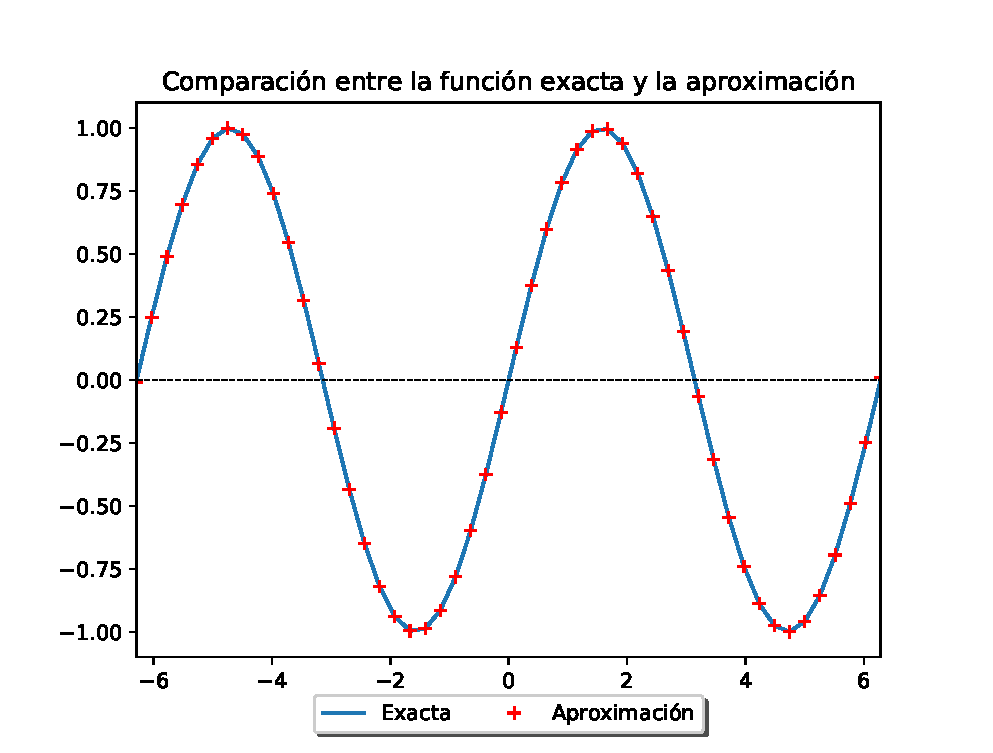
\includegraphics[scale=0.6]{Imagenes/Aproximacion_Seno.eps}
\end{figure}
\end{frame}
\end{document}